% Template for Cogsci submission with R Markdown

% Stuff changed from original Markdown PLOS Template
\documentclass[10pt, letterpaper]{article}

\usepackage{cogsci}
\usepackage{pslatex}
\usepackage{float}
\usepackage{caption}

% amsmath package, useful for mathematical formulas
\usepackage{amsmath}

% amssymb package, useful for mathematical symbols
\usepackage{amssymb}

% hyperref package, useful for hyperlinks
\usepackage{hyperref}

% graphicx package, useful for including eps and pdf graphics
% include graphics with the command \includegraphics
\usepackage{graphicx}

% Sweave(-like)
\usepackage{fancyvrb}
\DefineVerbatimEnvironment{Sinput}{Verbatim}{fontshape=sl}
\DefineVerbatimEnvironment{Soutput}{Verbatim}{}
\DefineVerbatimEnvironment{Scode}{Verbatim}{fontshape=sl}
\newenvironment{Schunk}{}{}
\DefineVerbatimEnvironment{Code}{Verbatim}{}
\DefineVerbatimEnvironment{CodeInput}{Verbatim}{fontshape=sl}
\DefineVerbatimEnvironment{CodeOutput}{Verbatim}{}
\newenvironment{CodeChunk}{}{}

% cite package, to clean up citations in the main text. Do not remove.
\usepackage{apacite}

% KM added 1/4/18 to allow control of blind submission
\cogscifinalcopy

\usepackage{color}

% Use doublespacing - comment out for single spacing
%\usepackage{setspace}
%\doublespacing


% % Text layout
% \topmargin 0.0cm
% \oddsidemargin 0.5cm
% \evensidemargin 0.5cm
% \textwidth 16cm
% \textheight 21cm

\title{When \emph{doggy} becomes \emph{dog}: Developmental shifts in
children's use of register-specific words}

\usepackage{booktabs}
\usepackage{longtable}
\usepackage{array}
\usepackage{multirow}
\usepackage{wrapfig}
\usepackage{float}
\usepackage{colortbl}
\usepackage{pdflscape}
\usepackage{tabu}
\usepackage{threeparttable}
\usepackage{threeparttablex}
\usepackage[normalem]{ulem}
\usepackage{makecell}
\usepackage{xcolor}

\author{{\large \bf Kennedy Casey} \\ University of Chicago \\ \texttt{kbcasey@uchicago.edu} \And {\large \bf Marisa Casillas} \\ University of Chicago \\ \texttt{mcasillas@uchicago.edu}}

\newlength{\cslhangindent}
\setlength{\cslhangindent}{1.5em}
\newenvironment{CSLReferences}%
  {}%
  {\par}

\begin{document}

\maketitle

\begin{abstract}
Child-directed language (CDL) features words such as \emph{doggy},
\emph{night-night}, and \emph{tummy} that are rarely used in
adult-directed language (ADL). Characterisitcs of CDL word forms, such
as diminutivization and reduplication, explain why they may be learned
and produced earlier by children. However, it is not yet clear how or
when children switch to using ADL equivalents---\emph{dog},
\emph{goodnight}, \emph{stomach}. Through analysis of speech transcripts
from CHILDES and the Language Development Project corpus, we show that
children significantly increase their production of ADL word forms
across age, with the average CDL-to-ADL transition point at 2.5 years.
Many of the linguistic features that distinguish CDL vs.~ADL registers
(e.g., lexical and syntactic complexity) similarly differentiated the
local speech contexts surrounding CDL vs.~ADL word forms. Learners may
therefore be able to capitalize on these cues to support their discovery
of register along with context-appropriate CDL/ADL pair use.

\textbf{Keywords:}
child-directed language; word production; linguistic input; social
register; corpus analysis; developmental change
\end{abstract}

\hypertarget{introduction}{%
\section{Introduction}\label{introduction}}

Across their first few years of life, children amass an impressive
expressive vocabulary, including hundreds if not thousands of words
(Fenson et al., 1994; Mayor \& Plunkett, 2011). Word production
typically begins around age one, followed by a vocabulary `explosion' or
`spurt' during toddlerhood (Ganger \& Brent, 2004; see also McMurray,
2007) and continued, measurable growth in vocabulary size thereafter
(Rice \& Hoffman, 2015).

\hypertarget{predictors-of-early-word-comprehension-and-production}{%
\subsection{Predictors of early word comprehension and
production}\label{predictors-of-early-word-comprehension-and-production}}

Which words do children understand and say first? Cross-linguistic
evidence points to a variety of statistical and semantic factors that
contribute to early learnability. For instance, words that are highly
frequent in children's input and words that appear in shorter or
isolated utterances are typically learned and produced earlier
(Braginsky, Yurovsky, Marchman, \& Frank, 2019). Concreteness predicts
earlier age of acquisition (Braginsky, Yurovsky, Marchman, \& Frank,
2019), but routine-based, social words also consistently appear among
infants' first words (Tardif et al., 2008). Words that adults rate as
more relevant for infants (e.g., \emph{bottle} and \emph{bib}, Perry,
Perlman, \& Lupyan, 2015) are typically understood earlier, and shorter
words with fewer phonemes are also produced earlier (Braginsky,
Yurovsky, Marchman, \& Frank, 2019).

Other features of word forms, such as iconicity (Laing, Vihman, \&
Keren-Portnoy, 2017), diminutivization (Kempe, Brooks, \& Gillis, 2005),
and reduplication (Ota, Davies-Jenkins, \& Skarabela, 2018), have been
shown to support children's early learning. Words with these features
(e.g., \emph{doggy} and \emph{choo-choo}) are typically overrepresented
in children's early productive vocabularies (e.g., Perry, Perlman,
Winter, Massaro, \& Lupyan, 2018) and serve as a hallmark of
child-directed language (CDL) across many communities (Ferguson, 1964).

In sum, children's productive vocabulary gets off the ground with many
words that are specifically tailored to them (i.e., affiliated
particularly with CDL). However, at some point--likely
gradually--children shift away from these baby-centric words. This
transition is perhaps most marked for common child language word forms
that have a direct substitute in adult language (e.g., \emph{doggy/dog},
\emph{tummy/stomach}, \emph{bunny/rabbit}) as opposed to words that
become less relevant over the years (e.g., \emph{diaper},
\emph{pacifier}, \emph{peekaboo}). Note, though, that these words do not
fully disappear---children themselves come to use these CDL-specific
words (along with other CDL features) when talking to infants and
younger children (REFS).

\hypertarget{comprehension-and-production-of-language-varieties}{%
\subsection{Comprehension and production of language
varieties}\label{comprehension-and-production-of-language-varieties}}

Classically, we might think of hearing multiple labels for the same
referent (e.g., \emph{doggy/dog}) as a problem for early word
learning---particularly for variants with little to no overlap in
phonological form (e.g., \emph{tummy/stomach}, or \emph{bunny/rabbit}).
There is abundant lab-based evidence for children's use of a mutual
exclusivity (ME) heuristic when learning new words; they assume that new
labels refer to new items rather than synonyms for words they already
know (Markman \& Wachtel, 1988; see Lewis, Cristiano, Lake, Kwan, \&
Frank, 2020, for a recent meta-analysis). Moreover, the existence of
multiple labels seems to contradict the idea that that features of
language should not be redundant (Clark \& MacWhinney, 1987).

Despite the theoretical problem that CDL-specific words may pose from a
conventional lens, children seem to make sense of multiple variants
without issue. One possible way to explain this is to think about the
social context of language use. Children's tendency to show the ME
effect is modulated by their experience with multiple languages (and
thus multiple labels: Byers-Heinlein \& Werker, 2009; Houston-Price,
Caloghiris, \& Raviglione, 2010) and the social conditions under which
multiple labels are introduced (e.g., by speakers of familiar or
unfamiliar race: Weatherhead, Kandhadai, Hall, \& Werker, 2021) To test
this idea, we first need to establish (a) when children begin to shift
away from producing CDL-specific words, and (b) how children may be able
to use bottom-up linguistic input cues to associate lexical variants
with their appropriate registers (i.e., CDL vs.~ADL).

Learners encounter many forms of socially meaningful variation in their
linguistic input -- different speakers (Bulgarelli \& Bergelson, 2021;
Rost \& McMurray, 2009), accents (Buckler, Oczak-Arsic, Siddiqui, \&
Johnson, 2017; Potter \& Saffran, 2017), dialects (Durrant, Delle Luche,
Cattani, \& Floccia, 2015; Edwards et al., 2014), languages (Kremin,
Alves, Orena, Polka, \& Byers-Heinlein, 2020), and registers (e.g., CDL
vs.~ADL, Bunce et al., 2020; Loukatou, Scaff, Demuth, Cristia, \&
Havron, 2021) -- all of which shape their ability to detect and learn
from such variation (see Johnson \& White, 2020, for a recent review).
Over time, children become increasingly aware that language style is
modulated by a variety of social factors, including the identities of
speakers (Liberman, Woodward, \& Kinzler, 2017) along with their
addressees (e.g., young children vs.~adults: Soley \& Sebastian-Galles,
2020). {[}need a transition here{]}

We hypothesize that one way that children may be able to make sense of
this otherwise redundant appearance of CDL-specific words with
straightforward ADL equivalents is to already begin associating them
with different modes of use (i.e., incipient representations of
register). {[}Also missing a transition here{]}. In this way, we should
view children's vocabulary development not as a simple accumulation of
words but rather a deepening and restructuring of the lexicon with
growing linguistic and social maturity. The word \emph{dog} does not
entirely replace \emph{doggy}---rather, the two forms become reserved
for use with different addressees. To test this idea, we first need to
establish (a) when children begin to shift away from producing
CDL-specific words, and (b) how children may be able to use bottom-up
linguistic input cues to associate lexical variants with their
appropriate registers (i.e., CDL vs.~ADL).

\hypertarget{current-investigation}{%
\subsection{Current investigation}\label{current-investigation}}

In the present work, we examine a core subset of 15 CDL-specific words
in English (e.g., \emph{doggy}, \emph{night-night}, \emph{tummy}) that
are prevalent in children's early vocabularies but are eventually
`replaced' by ADL words---\emph{dog}, \emph{goodnight}, \emph{stomach}.
In Study 1, we analyze over XXXX utterances of spontaneous speech from
children up to 7 years of age to establish when ADL forms become more
dominant in children's own productions. That is, when do children
`switch' from using CDL-associated to ADL-associated forms?

After establishing that the average age of `switchover' occurs around
2.5 years, we next explored children's input. We investigated the extent
to which CDL and ADL words are used in distinct linguistic contexts.
Further processing of XXXX adult utterances reveal that CDL and ADL
variants co-occur with reliably different patterns of prosodic, lexical,
and syntactic information---cues that likely help learners associate
them with different modes of use, or emerging representations of
register.

\hypertarget{study-1-when-do-children-shift-from-cdl-to-adl-forms}{%
\section{Study 1: When do children shift from CDL to ADL
forms?}\label{study-1-when-do-children-shift-from-cdl-to-adl-forms}}

We tracked children's use of 15 CDL/ADL word pairs (Table
\ref{tab:tab1}) from early infancy up to age seven. Since CDL forms
rarely appear in ADL, we predicted that children would shift away from
production of these register-specific forms with increasing age. That
is, we expected to see `replacement' of CDL forms with ADL forms in
children's own speech across time.

\hypertarget{method}{%
\section{Method}\label{method}}

\hypertarget{corpora}{%
\subsection{Corpora}\label{corpora}}

We analyzed 8251 transcripts in the North American English collection of
the Child Language Data Exchange System (CHILDES) database (MacWhinney,
2000) for children up to 7 years of age. The included transcripts were
drawn from 52 individual corpora and featured 980 children (age range =
1--84 months, \emph{M} = 33.5 months). Child production data from the
Language Development Project longitudinal corpus were also analyzed
(Huttenlocher, Waterfall, Vasilyeva, Vevea, \& Hedges, 2010, for further
details regarding participating families, recording procedures, and
transcription; see Rowe, 2008). These included 622 transcripts from 59
English-learning children recorded every 4 months for approximately 90
minutes from age 14 to 58 months.

\hypertarget{target-words}{%
\subsection{Target words}\label{target-words}}

Fifteen CDL/ADL word pairs (30 total target words) were selected based
on two criteria: the appearance of at least one form on the
MacArthur-Bates Communicative Development Inventory (CDI, Fenson et al.,
1994), and sufficient frequency of occurrence in CHILDES (at least 100
child-produced tokens and 100 other-produced tokens per form). Pairs
were also selected based on researcher intuition to ensure that the same
object, animal, routine, or body part could be reasonably labeled with
either form by young children.

\begin{table}[ht]
\centering
\resizebox{\linewidth}{!}{
\begin{tabular}{rlrrrr}
  \toprule
\multicolumn{2}{c}{\textbf{ }} & \multicolumn{2}{c}{\textbf{CDL tokens by speaker}} & \multicolumn{2}{c}{\textbf{ADL tokens by speaker}} \\
\cmidrule(l{3pt}r{3pt}){3-4} \cmidrule(l{3pt}r{3pt}){5-6}
\textbf{} & \textbf{Pair} & \textbf{Child} & \textbf{Other} & \textbf{Child} & \textbf{Other }\\ 
  \midrule
1 & doggy/dog & 2249 & 2644 & 3519 & 5113 \\ 
  2 & kitty/cat & 1552 & 3309 & 2779 & 4443 \\ 
  3 & tummy/stomach & 435 & 623 & 112 & 360 \\ 
  4 & daddy/dad & 9603 & 10048 & 2313 & 1031 \\ 
  5 & mommy/mom & 20294 & 17070 & 7616 & 2552 \\ 
  6 & bunny/rabbit & 1237 & 2597 & 1060 & 1397 \\ 
  7 & duckie/duck & 307 & 647 & 1933 & 3003 \\ 
  8 & blankie/blanket & 174 & 224 & 825 & 874 \\ 
  9 & froggy/frog & 154 & 434 & 970 & 1846 \\ 
  10 & potty/bathroom & 511 & 786 & 161 & 270 \\ 
  11 & night night/goodnight & 149 & 153 & 102 & 446 \\ 
  12 & dolly/doll & 745 & 1054 & 674 & 2697 \\ 
  13 & horsey/horse & 1149 & 1034 & 1749 & 2575 \\ 
  14 & piggy/pig & 405 & 1212 & 1276 & 2139 \\ 
  15 & birdie/bird & 399 & 588 & 1879 & 3358 \\ 
   \bottomrule
\end{tabular}}
\caption{CHILDES frequency for 15 CDL/ADL word pairs. Child-produced
                             counts include tokens produced only by the target child.} 
\label{tab:tab1}
\end{table}

\hypertarget{results}{%
\section{Results}\label{results}}

We first asked when CDL forms are `replaced' by ADL forms in children's
own speech. We fit a mixed-effects binomial logistic regression model
predicting children's production of CDL vs.~ADL forms, with target child
age (in months, scaled) as a single fixed effect. Random slopes and
intercepts for word pairs were also included. For each target word
token, the form was coded as either 0 (CDL) or 1 (ADL). Thus, the model
captures, for each age, the relative proportion of CDL vs.~ADL forms in
children's own speech.

Children's production of ADL forms increased with age (\(\beta\) = 0.54,
\emph{SE} = 0.11, \emph{t} = 4.92, \emph{p} \textless{} 0.001). This
trend of increasing ADL form production was significant for 13 of 15
pairs. The average CDL-to-ADL transition point (i.e., the point at which
ADL forms were produced \textgreater50\% of the time) was between 24 and
36 months of age (Figure 1).

\begin{CodeChunk}
\begin{figure}[h]

{\centering 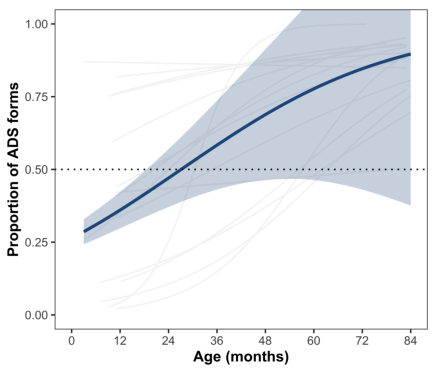
\includegraphics{figs/shift-timing-fig-1} 

}

\caption[Model-predicted increase in production of ADL forms with age]{Model-predicted increase in production of ADL forms with age. Gray lines depict individual word-pair trajectories.}\label{fig:shift-timing-fig}
\end{figure}
\end{CodeChunk}

\begin{CodeChunk}
\begin{figure*}[!ht]

{\centering 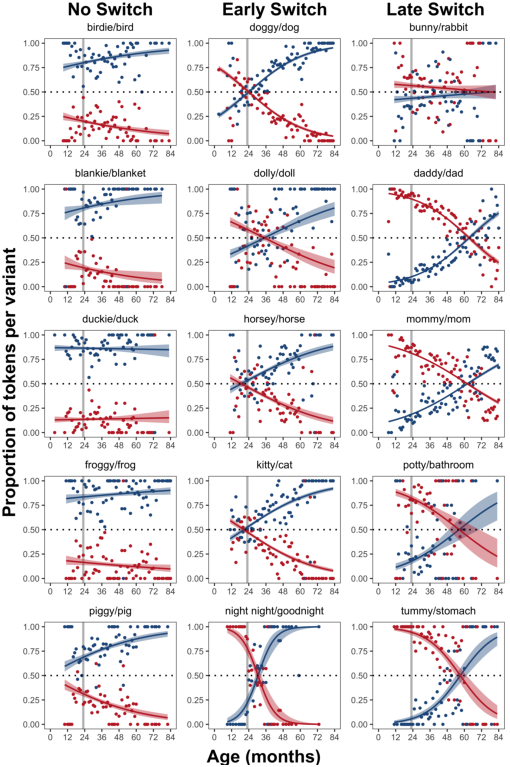
\includegraphics{figs/shift-timing-bypair-fig-1} 

}

\caption[Inidividual word-pair trajectories for increasing production of ADL forms (blue) and descreasing production of CDL forms (red) with age]{Inidividual word-pair trajectories for increasing production of ADL forms (blue) and descreasing production of CDL forms (red) with age. Points indicate proportions for each 1-month age bin.}\label{fig:shift-timing-bypair-fig}
\end{figure*}
\end{CodeChunk}

\hypertarget{discussion}{%
\section{Discussion}\label{discussion}}

\hypertarget{study-2-what-linguisitc-information-in-childrens-input-supports-their-shift-from-cdl-to-adl-forms}{%
\section{Study 2: What linguisitc information in children's input
supports their shift from CDL to ADL
forms?}\label{study-2-what-linguisitc-information-in-childrens-input-supports-their-shift-from-cdl-to-adl-forms}}

We next explored children's input (i.e., other-produced speech), asking
whether the linguistic features that differentiate CDL vs.~ADL at the
register level also differentiate the local speech contexts surrounding
CDL vs.~ADL forms. In other words, can form be predicted on the basis of
individual utterance-level prosodic, lexical, or syntactic cues?

\begin{CodeChunk}
\begin{figure*}[h]

{\centering 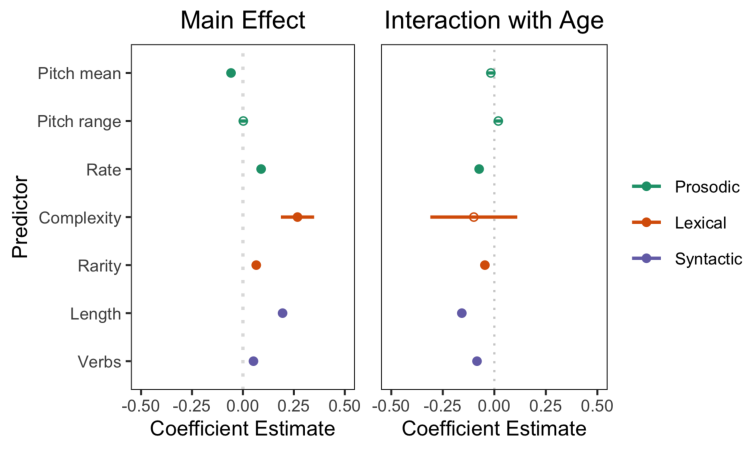
\includegraphics{figs/ling-predictors-fig-1} 

}

\caption[Coefficient estimates for linguistic predictors of form]{Coefficient estimates for linguistic predictors of form. Positive main effects indicate that utterances are more likely to contain ADL forms when they have higher values for the predictor (e.g., faster speech rates). Positive age interactions indicate an increasing effect of the predictor with age. Error bars depict standard errors of the coefficient estimates, and filled circles represent significant effects (\textit{p} $<$ 0.05).}\label{fig:ling-predictors-fig}
\end{figure*}
\end{CodeChunk}

\hypertarget{method-1}{%
\section{Method}\label{method-1}}

\hypertarget{corpora-1}{%
\subsection{Corpora}\label{corpora-1}}

We analyzed XXXX other-produced utterances (i.e., utterances not
produced by the target child) in the same CHILDES transcripts from Study
1. The majority were utterances from primary caregivers (XX\%).

\hypertarget{linguistic-input-predictors}{%
\subsection{Linguistic input
predictors}\label{linguistic-input-predictors}}

All input analyses were conducted over individual utterances containing
one of the 30 target words from Study 1. We quantified prosodic,
lexical, and syntactic information to describe each utterance.

\hypertarget{prosodic-level}{%
\subsubsection{Prosodic level}\label{prosodic-level}}

We measured three types of prosodic information: \textbf{mean pitch}
(Hz), \textbf{pitch range} (Hz), and \textbf{speech rate} (words per
second). These measures were calculated over all timestamped utterances
in CHILDES (42.3\% of other-produced utterances). Utterances shorter
than 58 ms were excluded from analysis. This lower bound was set by
identifying the the shortest possible duration of an utterance
containing at least one word in four manually annotated North American
English corpora in HomeBank (Bergelson, 2016; McDivitt \& Soderstrom,
2016; VanDam et al., 2016; VanDam, 2016; Warlaumont \& Pretzer, 2016) .
Pitch information was extracted using Praat software (Boersma \&
Weenink, 2016).

\hypertarget{lexical-level}{%
\subsubsection{Lexical level}\label{lexical-level}}

We measured two types of lexical information: complexity and rarity.
\textbf{Lexical complexity} was defined as the negative log proportion
of known words in each utterance (consistent with Foushee, Griffiths, \&
Srinivasan, 2016; Kidd, Piantadosi, \& Aslin, 2012). A word was
considered `known' if the age of acquisition (AoA) estimate (Fenson et
al., 1994; Frank, Braginsky, Yurovsky, \& Marchman, 2017) was less than
or equal to the age of the target child when they heard the utterance.
Utterances with proportionally fewer known words are more lexically
complex. \textbf{Lexical rarity} was determined based on overall
frequency in CHILDES. For all words with at least 10 tokens\footnote{Manual
  checks revealed that many of the lowest-frequency words included
  idiosyncratic or erroneous transcriptions.}, we calculated a rarity
score as the negative log proportion of other-produced tokens in CHILDES
(i.e., number of tokens for a given word/sum of all tokens in the full
corpus), and then averaged for rarity scores for all target utterances.
Utterances with more low-frequency words are considered more lexically
rare.

\hypertarget{syntactic-level}{%
\subsubsection{Syntactic level}\label{syntactic-level}}

Syntactic measures included both the utterance \textbf{length} (in
words) and \textbf{number of verb phrases}. The number of words per
utterance was automatically extracted using the \texttt{childesr}
package (Braginsky, Sanchez, \& Yurovsky, 2021). The number of verb
phrases per utterance was determined using \texttt{spaCy3}, an automatic
syntactic parser (Honnibal, Montani, Van Landeghem, \& Boyd, 2020).

\hypertarget{results-1}{%
\section{Results}\label{results-1}}

We ran individual mixed-effects binomial logistic regression models for
each of seven linguisitc input predictors. Models included fixed effects
of linguistic predictor, target child age, and their interaction as well
as random intercepts for individual word pairs and speakers. For each
target word token, form was coded as CDL (0) or ADL (1), so coefficient
estimates should be interpreted as an indication of the likelihood that
an utterance contains an ADL form. All main effects of linguistic
predictors and interactions with age are shown in Figure 3.

At the prosodic level, we found significant effects for two of three
input predictors tested. Utterance-level \textbf{pitch range} was not
predictive of form (\(\beta\) = 0.002, \emph{SE} = 0.02, \emph{t} = 0.1,
\emph{p} = 0.919) and did not significantly interact with age (\(\beta\)
= 0.02, \emph{SE} = 0.02, \emph{t} = 1.11, \emph{p} = 0.268). However,
utterance-level \textbf{mean pitch} was a negative predictor of ADL form
(\(\beta\) = -0.058, \emph{SE} = 0.02, \emph{t} = -3.02, \emph{p} =
0.003). That is, utterances with higher overall mean pitch were more
likely to contain CDL forms, with no significant interaction with age
(\(\beta\) = -0.02, \emph{SE} = 0.02, \emph{t} = -0.96, \emph{p} =
0.337). \textbf{Speech rate} (i.e., words produced per second) was a
positive predictor of ADL form (\(\beta\) = 0.09, \emph{SE} = 0.02,
\emph{t} = 4.86, \emph{p} \textless{} 0.001). Utterances spoken more
quickly were more likely to contain ADL forms. This input predictor also
negatively interacted with age (\(\beta\) = -0.07, \emph{SE} = 0.02,
\emph{t} = -3.96, \emph{p} \textless{} 0.001), indicating a decreasing
strength in predictive power across developmental time.

At the lexical level, we found significant effects for both input
predictors tested. Utterances with higher levels of \textbf{lexical
complexity} (\(\beta\) = 0.27, \emph{SE} = 0.08, \emph{t} = 3.28,
\emph{p} = 0.001) and \textbf{lexical rarity} (\(\beta\) = 0.07,
\emph{SE} = 0.01, \emph{t} = 5.73, \emph{p} \textless{} 0.001) were more
likely to contain ADL forms. Lexical complexity did not interact with
age (\(\beta\) = -0.1, \emph{SE} = 0.21, \emph{t} = -0.47, \emph{p} =
0.637); whereas, lexical rarity negatively interacted with age such that
there was a decreasing effect of this predictor with age (\(\beta\) =
-0.05, \emph{SE} = 0.01, \emph{t} = -3.95, \emph{p} \textless{} 0.001).

At the syntactic level, we found significant effects of
\textbf{utterance length} and \textbf{number of verb phrases}.
Utterances with more words (\(\beta\) = 0.19, \emph{SE} = 0.01, \emph{t}
= 16.3, \emph{p} \textless{} 0.001) and more verb phrases (\(\beta\) =
0.05, \emph{SE} = 0.01, \emph{t} = 4.44, \emph{p} \textless{} 0.001)
were more likely to contain ADL forms. Moreover, both linguistic
predictors negatively interacted with age (Length: \(\beta\) = -0.16,
\emph{SE} = 0.01, \emph{t} = -14.61, \emph{p} \textless{} 0.001; Verbs:
\(\beta\) = -0.08, \emph{SE} = 0.01, \emph{t} = -7.7, \emph{p}
\textless{} 0.001), suggesting that the strength of these predictors
decreases across developmental time.

\hypertarget{possible-section-talking-about-how-some-of-these-patterns-are-mirrored-in-childrens-own-speech}{%
\subsection{Possible section talking about how some of these patterns
are mirrored in children's own
speech}\label{possible-section-talking-about-how-some-of-these-patterns-are-mirrored-in-childrens-own-speech}}

\hypertarget{discussion-1}{%
\section{Discussion}\label{discussion-1}}

\hypertarget{general-discussion}{%
\section{General Discussion}\label{general-discussion}}

Para about how we don't yet know which (if any of these) linguistic cues
are actually exploited by learners (\textbf{potter2019infants?} as a
good ref). However, the current work sets us up to be able to test some
of these ideas experimentally. Additional point that CDL and ADL
registers are differentiated by more than just linguistic cues, so we
can think about whether the same happens for CDL vs.~ADL forms.

Para on ties to other sociolinguistic phenomena, like dialects, accents,
and other types of register (e.g., pedagogical, narrative, etc.).
Learning happening at multiple levels -- not just words but associations
between words and surrounding context (linguistic, social, etc.).

Maybe some critique of typical caregiver-report measures, like CDIs,
that gloss over lexical variation. Standardization makes sense for some
things, but we lose the opportunity to capture deepening linguistic
knowledge

\hypertarget{references}{%
\section{References}\label{references}}

\setlength{\parindent}{-0.1in} 
\setlength{\leftskip}{0.125in}

\noindent

\hypertarget{refs}{}
\begin{CSLReferences}{1}{0}
\leavevmode\hypertarget{ref-bergelsoncorpus}{}%
Bergelson, E. (2016). Bergelson HomeBank corpus.
\url{https://doi.org/10.21415/T5PK6D}.

\leavevmode\hypertarget{ref-boersma2016praat}{}%
Boersma, P., \& Weenink, D. (2016). Praat software. \emph{Amsterdam:
University of Amsterdam}.

\leavevmode\hypertarget{ref-braginsky2021childesr}{}%
Braginsky, M., Sanchez, A., \& Yurovsky, D. (2021). \emph{Childesr:
Accessing the 'CHILDES' database}. Retrieved from
\url{https://CRAN.R-project.org/package=childesr}

\leavevmode\hypertarget{ref-braginsky2019consistency}{}%
Braginsky, M., Yurovsky, D., Marchman, V. A., \& Frank, M. C. (2019).
Consistency and variability in children's word learning across
languages. \emph{Open Mind}, \emph{3}, 52--67.

\leavevmode\hypertarget{ref-buckler2017input}{}%
Buckler, H., Oczak-Arsic, S., Siddiqui, N., \& Johnson, E. K. (2017).
Input matters: Speed of word recognition in 2-year-olds exposed to
multiple accents. \emph{Journal of Experimental Child Psychology},
\emph{164}, 87--100.

\leavevmode\hypertarget{ref-bulgarelli2021talker}{}%
Bulgarelli, F., \& Bergelson, E. (2021). Talker variability shapes early
word representations in english-learning 8-month-olds. \emph{Infancy}.

\leavevmode\hypertarget{ref-bunceURcross}{}%
Bunce, J., Soderstrom, M., Bergelson, E., Rosemberg, C., Stein, A.,
Migdalek, M., \ldots{} others. (2020). A cross-cultural examination of
young children's everyday language experiences.

\leavevmode\hypertarget{ref-byers2009monolingual}{}%
Byers-Heinlein, K., \& Werker, J. F. (2009). Monolingual, bilingual,
trilingual: Infants' language experience influences the development of a
word-learning heuristic. \emph{Developmental Science}, \emph{12}(5),
815--823.

\leavevmode\hypertarget{ref-clark1987principle}{}%
Clark, E. V., \& MacWhinney, B. (1987). The principle of contrast: A
constraint on language acquisition. \emph{Mechanisms of Language
Acquisition}, 1--33.

\leavevmode\hypertarget{ref-durrant2015monodialectal}{}%
Durrant, S., Delle Luche, C., Cattani, A., \& Floccia, C. (2015).
Monodialectal and multidialectal infants' representation of familiar
words. \emph{Journal of Child Language}, \emph{42}(2), 447--465.

\leavevmode\hypertarget{ref-edwards2014dialect}{}%
Edwards, J., Gross, M., Chen, J., MacDonald, M. C., Kaplan, D., Brown,
M., \& Seidenberg, M. S. (2014). Dialect awareness and lexical
comprehension of mainstream american english in african american
english--speaking children. \emph{Journal of Speech, Language, and
Hearing Research}, \emph{57}(5), 1883--1895.

\leavevmode\hypertarget{ref-fenson1994variability}{}%
Fenson, L., Dale, P. S., Reznick, J. S., Bates, E., Thal, D. J.,
Pethick, S. J., \ldots{} Stiles, J. (1994). Variability in early
communicative development. \emph{Monographs of the Society for Research
in Child Development}, i--185.

\leavevmode\hypertarget{ref-ferguson1964baby}{}%
Ferguson, C. A. (1964). Baby talk in six languages. \emph{American
Anthropologist}, \emph{66}(6\_PART2), 103--114.

\leavevmode\hypertarget{ref-foushee2016lexical}{}%
Foushee, R., Griffiths, T., \& Srinivasan, M. (2016). Lexical complexity
of child-directed and overheard speech: Implications for learning. In
\emph{Proceedings of the 38th annual conference of the cognitive science
society} (pp. 1697--1702).

\leavevmode\hypertarget{ref-frank2017wordbank}{}%
Frank, M. C., Braginsky, M., Yurovsky, D., \& Marchman, V. A. (2017).
Wordbank: An open repository for developmental vocabulary data.
\emph{Journal of Child Language}, \emph{44}(3), 677--694.

\leavevmode\hypertarget{ref-ganger2004reexamining}{}%
Ganger, J., \& Brent, M. R. (2004). Reexamining the vocabulary spurt.
\emph{Developmental Psychology}, \emph{40}(4), 621.

\leavevmode\hypertarget{ref-honnibal2020spacy}{}%
Honnibal, M., Montani, I., Van Landeghem, S., \& Boyd, A. (2020).
{spaCy: Industrial-strength Natural Language Processing in Python}.
http://doi.org/\href{https://doi.org/10.5281/zenodo.1212303}{10.5281/zenodo.1212303}

\leavevmode\hypertarget{ref-houston2010language}{}%
Houston-Price, C., Caloghiris, Z., \& Raviglione, E. (2010). Language
experience shapes the development of the mutual exclusivity bias.
\emph{Infancy}, \emph{15}(2), 125--150.

\leavevmode\hypertarget{ref-huttenlocher2010sources}{}%
Huttenlocher, J., Waterfall, H., Vasilyeva, M., Vevea, J., \& Hedges, L.
V. (2010). Sources of variability in children's language growth.
\emph{Cognitive Psychology}, \emph{61}(4), 343--365.

\leavevmode\hypertarget{ref-johnson2020developmental}{}%
Johnson, E. K., \& White, K. S. (2020). Developmental sociolinguistics:
Children's acquisition of language variation. \emph{Wiley
Interdisciplinary Reviews: Cognitive Science}, \emph{11}(1), e1515.

\leavevmode\hypertarget{ref-kempe2005diminutives}{}%
Kempe, V., Brooks, P. J., \& Gillis, S. (2005). Diminutives in
child-directed speech supplement metric with distributional word
segmentation cues. \emph{Psychonomic Bulletin \& Review}, \emph{12}(1),
145--151.

\leavevmode\hypertarget{ref-kidd2012goldilocks}{}%
Kidd, C., Piantadosi, S. T., \& Aslin, R. N. (2012). The goldilocks
effect: Human infants allocate attention to visual sequences that are
neither too simple nor too complex. \emph{PloS One}, \emph{7}(5),
e36399.

\leavevmode\hypertarget{ref-kremin2020code}{}%
Kremin, L. V., Alves, J., Orena, A. J., Polka, L., \& Byers-Heinlein, K.
(2020). Code-switching in parents' everyday speech to bilingual infants.
\emph{Journal of Child Language}, 1--27.

\leavevmode\hypertarget{ref-laing2017salient}{}%
Laing, C. E., Vihman, M., \& Keren-Portnoy, T. (2017). How salient are
onomatopoeia in the early input? A prosodic analysis of infant-directed
speech. \emph{Journal of Child Language}, \emph{44}(5), 1117--1139.

\leavevmode\hypertarget{ref-lewis2020role}{}%
Lewis, M., Cristiano, V., Lake, B. M., Kwan, T., \& Frank, M. C. (2020).
The role of developmental change and linguistic experience in the mutual
exclusivity effect. \emph{Cognition}, \emph{198}, 104191.

\leavevmode\hypertarget{ref-liberman2017preverbal}{}%
Liberman, Z., Woodward, A. L., \& Kinzler, K. D. (2017). Preverbal
infants infer third-party social relationships based on language.
\emph{Cognitive Science}, \emph{41}, 622--634.

\leavevmode\hypertarget{ref-loukatou2021child}{}%
Loukatou, G., Scaff, C., Demuth, K., Cristia, A., \& Havron, N. (2021).
Child-directed and overheard input from different speakers in two
distinct cultures. \emph{Journal of Child Language}, 1--20.

\leavevmode\hypertarget{ref-macwhinney2000childes}{}%
MacWhinney, B. (2000). \emph{The CHILDES project: The database} (Vol.
2). Psychology Press.

\leavevmode\hypertarget{ref-markman1988children}{}%
Markman, E. M., \& Wachtel, G. F. (1988). Children's use of mutual
exclusivity to constrain the meanings of words. \emph{Cognitive
Psychology}, \emph{20}(2), 121--157.

\leavevmode\hypertarget{ref-mayor2011statistical}{}%
Mayor, J., \& Plunkett, K. (2011). A statistical estimate of infant and
toddler vocabulary size from CDI analysis. \emph{Developmental Science},
\emph{14}(4), 769--785.

\leavevmode\hypertarget{ref-soderstromcorpus}{}%
McDivitt, K., \& Soderstrom, M. (2016). McDivitt HomeBank corpus.
\url{https://doi.org/10.21415/T5KK6G}.

\leavevmode\hypertarget{ref-mcmurray2007defusing}{}%
McMurray, B. (2007). Defusing the childhood vocabulary explosion.
\emph{Science}, \emph{317}(5838), 631--631.

\leavevmode\hypertarget{ref-ota2018choo}{}%
Ota, M., Davies-Jenkins, N., \& Skarabela, B. (2018). Why choo-choo is
better than train: The role of register-specific words in early
vocabulary growth. \emph{Cognitive Science}, \emph{42}(6), 1974--1999.

\leavevmode\hypertarget{ref-perry2015iconicity}{}%
Perry, L. K., Perlman, M., \& Lupyan, G. (2015). Iconicity in english
and spanish and its relation to lexical category and age of acquisition.
\emph{PloS One}, \emph{10}(9), e0137147.

\leavevmode\hypertarget{ref-perry2018iconicity}{}%
Perry, L. K., Perlman, M., Winter, B., Massaro, D. W., \& Lupyan, G.
(2018). Iconicity in the speech of children and adults.
\emph{Developmental Science}, \emph{21}(3), e12572.

\leavevmode\hypertarget{ref-potter2017exposure}{}%
Potter, C. E., \& Saffran, J. R. (2017). Exposure to multiple accents
supports infants' understanding of novel accents. \emph{Cognition},
\emph{166}, 67--72.

\leavevmode\hypertarget{ref-rice2015predicting}{}%
Rice, M. L., \& Hoffman, L. (2015). Predicting vocabulary growth in
children with and without specific language impairment: A longitudinal
study from 2; 6 to 21 years of age. \emph{Journal of Speech, Language,
and Hearing Research}, \emph{58}(2), 345--359.

\leavevmode\hypertarget{ref-rost2009speaker}{}%
Rost, G. C., \& McMurray, B. (2009). Speaker variability augments
phonological processing in early word learning. \emph{Developmental
Science}, \emph{12}(2), 339--349.

\leavevmode\hypertarget{ref-rowe2008child}{}%
Rowe, M. L. (2008). Child-directed speech: Relation to socioeconomic
status, knowledge of child development and child vocabulary skill.
\emph{Journal of Child Language}, \emph{35}(1), 185--205.

\leavevmode\hypertarget{ref-soley2020infants}{}%
Soley, G., \& Sebastian-Galles, N. (2020). Infants' expectations about
the recipients of infant-directed and adult-directed speech.
\emph{Cognition}, \emph{198}, 104214.

\leavevmode\hypertarget{ref-tardif2008baby}{}%
Tardif, T., Fletcher, P., Liang, W., Zhang, Z., Kaciroti, N., \&
Marchman, V. A. (2008). Baby's first 10 words. \emph{Developmental
Psychology}, \emph{44}(4), 929.

\leavevmode\hypertarget{ref-vandamcorpus}{}%
VanDam, M. (2016). VanDam2 HomeBank corpus.

\leavevmode\hypertarget{ref-homebank}{}%
VanDam, M., Warlaumont, A. S., Bergelson, E., Cristia, A., De Palma, P.,
\& MacWhinney, B. (2016). Homebank: An online repository of daylong
child-centered audio recordings. \url{https://homebank.talkbank.org}.

\leavevmode\hypertarget{ref-warlaumontcorpus}{}%
Warlaumont, A. S., \& Pretzer, G. M. (2016). Warlaumont HomeBank corpus.
\url{https://doi.org/10.21415/t54s3c}.

\leavevmode\hypertarget{ref-weatherhead2021putting}{}%
Weatherhead, D., Kandhadai, P., Hall, D. G., \& Werker, J. F. (2021).
Putting mutual exclusivity in context: Speaker race influences
monolingual and bilingual infants' word-learning assumptions.
\emph{Child Development}, \emph{92}(5), 1735--1751.

\end{CSLReferences}

\bibliographystyle{apacite}


\end{document}
